\chapter{Search Algorithms}

\section{Uninformed Search}

\begin{center}
   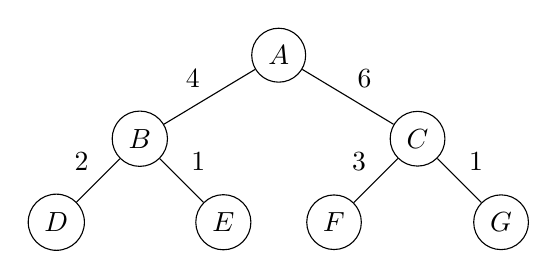
\begin{tikzpicture}
      [node distance=1.5cm, main node/.style={circle,draw,minimum size=6mm}]
      \node[main node] (a) at (0,0) {$A$};

      \node[main node, below left of=a, xshift=-2em] (b) {$B$};
      \node[main node, below right of=a, xshift=2em] (c) {$C$};
      
      \node[main node, below left of=b] (d) {$D$};
      \node[main node, below right of=b] (e) {$E$};
      
      \node[main node, below left of=c] (f) {$F$};
      \node[main node, below right of=c] (g) {$G$};

      \draw (a) -- node[above left] {4} (b) -- node[above left] {2} (d);
      \draw (a) -- node[above right] {6} (c) -- node[above right] {1} (g);
      \draw (b) -- node[above right] {1} (e);
      \draw (c) -- node[above left] {3} (f);
   \end{tikzpicture}
\end{center}

\subsection{Breadth-First Search (BFS)}
\begin{minipage}[t]{0.5\textwidth}
   \vspace{0pt}
   \begin{tabularx}{\textwidth}{|c|c|C|C|}\hline
      \thc{\#} & \thc{Node} &
      \thc{Closed Fringe} & \thc{Open Fringe}
      \\\hline
      1 & $A$ & $\{A\}$ & $\{B,C\}$\\\hline
      2 & $B$ & $\{A,B\}$ & $\{C,D,E\}$\\\hline
      3 & $C$ & $\{A,B,C\}$ & $\{D,E,F,G\}$\\\hline
      4 & $D$ & $\{A,B,C,D\}$ & $\{E,F,G\}$\\\hline
      5 & $E$ & $\{A,B,C,D,E\}$ & $\{F,G\}$\\\hline
      6 & $F$ & $\{A,B,C,D,E,F\}$ & $\{G\}$\\\hline
      7 & $G$ & $\{A,B,C,D,E,F,G\}$ & $\{ \ \}$\\\hline
   \end{tabularx}
\end{minipage}%
\hfill
\begin{minipage}[t]{0.48\textwidth}
   \vspace{0pt}
   \raggedright
   Explore nodes: $A,B,D,E,C,F,G$
\end{minipage}

\vspace{2em}
\subsection{Depth-First Search (DFS)}
\begin{minipage}[t]{0.5\textwidth}
\vspace{0pt}
\begin{tabularx}{\textwidth}{|c|c|C|C|}\hline
   \thc{\#} & \thc{Node} &
   \thc{Closed Fringe} & \thc{Open Fringe}
   \\\hline
   1 & $A$ & $\{A\}$ & $\{C,B\}$ \\\hline
   2 & $B$ & $\{A,B\}$ & $\{C,E,D\}$ \\\hline
   3 & $D$ & $\{A,B,D\}$ & $\{C,E\}$ \\\hline
   4 & $E$ & $\{A,B,D,E\}$ & $\{C\}$ \\\hline
   5 & $C$ & $\{A,B,D,E,C\}$ & $\{G,F\}$ \\\hline
   6 & $F$ & $\{A,B,D,E,C,F\}$ & $\{G\}$ \\\hline
   7 & $G$ & $\{A,B,D,E,C,F,G\}$ & $\{ \}$ \\\hline
\end{tabularx}
\end{minipage}%
\hfill
\begin{minipage}[t]{0.48\textwidth}
   \vspace{0pt}
   \raggedright
   Explore nodes: $A,B,D,E,C,F,G$
\end{minipage}


\begin{center}
   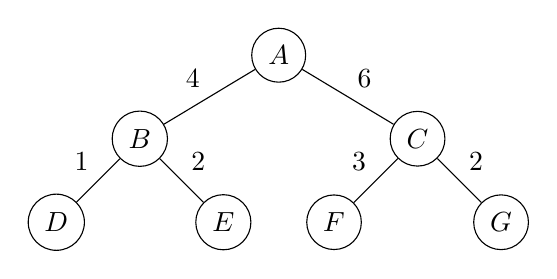
\begin{tikzpicture}
      [node distance=1.5cm, main node/.style={circle,draw,minimum size=6mm}]
      \node[main node] (a) at (0,0) {$A$};

      \node[main node, below left of=a, xshift=-2em] (b) {$B$};
      \node[main node, below right of=a, xshift=2em] (c) {$C$};
      
      \node[main node, below left of=b] (d) {$D$};
      \node[main node, below right of=b] (e) {$E$};
      
      \node[main node, below left of=c] (f) {$F$};
      \node[main node, below right of=c] (g) {$G$};

      \draw (a) -- node[above left] {4} (b) -- node[above left] {1} (d);
      \draw (a) -- node[above right] {6} (c) -- node[above right] {2} (g);
      \draw (b) -- node[above right] {2} (e);
      \draw (c) -- node[above left] {3} (f);
   \end{tikzpicture}
\end{center}

\vspace{1em}
\subsection{Iterative Deepening Search (IDS)}
% \begin{minipage}[t]{0.5\textwidth}
% \vspace{0pt}
% \begin{tabularx}{\textwidth}{|c|C|}\hline
%    \thc{Depth limit} & \thc{IDS (Nodes Visited in Order)} \\\hline
%    0 & $A$ \\\hline
%    1 & $A,B,C$ \\\hline
%    2 & $A,B,D,E,C,F,G$ \\\hline
% \end{tabularx}
% \end{minipage}%
% \hfill
% \begin{minipage}[t]{0.48\textwidth}
%    \vspace{0pt}
%    \raggedright
%    Explore nodes: $A,B,D,E,C,F,G$
% \end{minipage}

\begin{minipage}[t]{0.5\textwidth}
   \vspace{0pt}
\begin{tabularx}{\textwidth}{|c|C|}\hline
   \thc{Depth limit} & \thc{IDS (Nodes Visited in Order)} \\\hline
   1 & $A$ \\\hline
   2 & $\begin{array}{l}
      A \to B \\
      A \to C \\
   \end{array}$ \\\hline
   3 & $\begin{array}{l}
      A \to B \to D \\
      A \to B \to E\\
      A \to C \to F\\
      A \to C \to G\\
   \end{array}$ \\\hline
\end{tabularx}
\end{minipage}%
\hfill
\begin{minipage}[t]{0.48\textwidth}
   \vspace{0pt}
   \raggedright
   Explore nodes: $A,B,D,E,C,F,G$
\end{minipage}


\vspace{1em}
\subsection{Uniform Cost Search (UCS)}
\begin{minipage}[t]{0.5\textwidth}
   \vspace{0pt}
   \begin{tabularx}{\textwidth}{|c|c|C|C|}\hline
      \thc{\#} & \thc{Node} &
      \thc{Closed Fringe} & \thc{Open Fringe}
      \\\hline
      1 & $A$ & $\{A\}$ & $\{B(4), C(6)\}$ \\\hline
      2 & $B$ & $\{A,B\}$ & $\{C(6), D(5), E(6)\}$ \\\hline
      3 & $D$ & $\{A,B,D\}$ & $\{C(6), E(6)\}$ \\\hline
      4 & $C$ & $\{A,B,D,C\}$ & $\{E(6), F(9), G(8)\}$ \\\hline
      5 & $E$ & $\{A,B,D,C,E\}$ & $\{F(9), G(8)\}$ \\\hline
      6 & $G$ & $\{A,B,D,C,E,G\}$ & $\{F(9)\}$ \\\hline
      7 & $F$ & $\{A,B,D,C,E,G,F\}$ & $\{ \ \}$ \\\hline
   \end{tabularx}
\end{minipage}%
\hfill
\begin{minipage}[t]{0.48\textwidth}
   \vspace{0pt}
   \raggedright
   Explore nodes: $A,B,D,C,E,G,F$
\end{minipage}


\vspace{1em}
\subsection*{Summary of Uninformed Searching Algorithms}
\begin{tabularx}{\textwidth}{|l|L|L|L|L|}\hline
   \thc{Criteria} & \thc{BFS} & \thc{DFS} & \thc{IDS} & \thc{UCS} \\\hline
   Approach
   & BFS explores the graph level by level, visiting all nodes at the current depth before moving to the next.
   & DFS starts from the source, dives deep into one branch, and then backtracks to explore other branches.
   & Iteratively applies DFS with an increasing depth limit (0,1,2,…) until the goal is found.
   & Expands the node with the lowest path cost (not depth).
   \\\hline
   Data Structure & Queue & Stack & Stack + depth limit & Priority Queue\\\hline
   Complete? & Yes & No (if infinitely deep) & Yes & Yes (if costs are positive)\\\hline
   Optimal? & Yes & No & Yes & Yes \\\hline
   Time & $O(b^d)$ & $O(b^m)$ & $O(b^d)$ & $O(b^{C^*\varepsilon})$ \\\hline
   Space & $O(b^d)$ & $O(bm)$ & $O(bd)$ & $O(b^{C^*\varepsilon})$  \\\hline
\end{tabularx}

$b$: branching factor, \quad $d$: depth of the shallowest goal,
\quad $m$: max depth of search tree, \quad $C^*$ optimal cost,
\quad $\varepsilon$: smallest step cost.


\section{Informed Search}

\subsection{A* Search}

\begin{center}
\begin{minipage}{0.6\textwidth}
   \begin{tabular}{l}
      $h(S) =$ \ (43 mod 3) + 5 = 6 \\
      $h(A) =$ \ (43 mod 2) + 4 = 5 \\
      $h(B) =$ \ (43 mod 4) + 3 = 6 \\
      $h(C) =$ \ 5 + 2 = 7 \\
      $h(D) =$ \ 6 + 3 = 9
   \end{tabular}
\end{minipage}%
\begin{minipage}{0.4\textwidth}
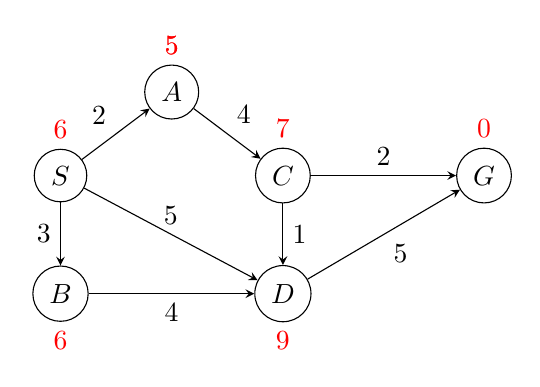
\begin{tikzpicture}
[node distance=1.5cm, main node/.style={circle,draw,minimum size=6mm},
every label/.style={red}]
\node[main node, label=above:{5}, label=above:{5}] (a) at (0,0) {$A$};
\node[main node, below left of=a, xshift=-1em, label=above:{6}] (s) {$S$};
\node[main node, below right of=a, xshift=1em, label=above:{7}] (c) {$C$};
\node[main node, below of=s, label=below:{6}] (b) {$B$};
\node[main node, below of=c, label=below:{9}] (d) {$D$};
\node[main node, right of=c, xshift=3em, label=above:{0}] (g) {$G$};

\draw[-stealth] (s) -- node[above left] {2} (a);
\draw[-stealth] (s) -- node[left] {3} (b);
\draw[-stealth] (s) -- node[above] {5} (d);

\draw[-stealth] (a) -- node[above right] {4} (c);
\draw[-stealth] (b) -- node[below] {4} (d);
\draw[-stealth] (c) -- node[right] {1} (d);

\draw[-stealth] (c) -- node[above] {2} (g);
\draw[-stealth] (d) -- node[below right] {5} (g);
\end{tikzpicture}
\end{minipage}
\end{center}

\vspace{2em}
\begin{tabularx}{\textwidth}{|c|C|c|c|c|X|X|}\hline
   Iteration & Path & $g(n)$ & $h(n)$
   & $\begin{array}{c}
      f(n) =\\[-0.5em]g(n) + h(n)
   \end{array}$ 
   & Closed Fringe & Open Fringe \\\hline
   
   Initialize & $\begin{array}{l}S\end{array}$ & 0 & 6 & 6
   & $\{ \ \}$ &  $\{S(6)\}$ \\\hline
   
   1
   & \makecell{$S \to A$\\$S \to B$\\$S \to D$}
   & \makecell{0+2 = 2\\0+3 = 3\\0+5 = 5} & \makecell{5\\6\\9}
   & \makecell{7\\9\\14}
   & $\{S\}$ &  $\{\ul[rgbRF]{A(7)},B(9),D(14)\}$\\\hline
   
   2
   & \makecell{$S \to A \to C$}
   & \makecell{2+4 = 6} & \makecell{7}
   & \makecell{13}
   & $\{S,A\}$ &  $\{\ul[rgbRF]{B(9)},D(14),C(13)\}$\\\hline
   
   3
   & \makecell{$S \to B \to D$}
   & \makecell{3+4 = 7} & \makecell{9}
   & \makecell{16}
   & $\{S,A,B\}$ &  $\{D(14),C(13)\}$\\\hline
   
   4
   & \makecell{$S \to A \to C \to D$\\$S \to A \to C \to G$}
   & \makecell{6+1 = 7\\6+2=8} & \makecell{9\\0}
   & \makecell{16\\8}
   & $\{S,A,B\}$ &  $\{D(14),G(0)\}$\\\hline
\end{tabularx}

\pagebreak
\begin{center}
\begin{minipage}{0.6\textwidth}
\begin{tabular}{l}
$h(S) =$ \ (Last 2 digits of id \% 2) + 1 \ = \ (43 \% 2) + 1 \ = \ 2\\
$h(A) =$ \ (Last 2 digits of id \% 3) + 2 \ = \ (43 \% 3) + 2 \ = \ 3\\
$h(B) =$ \ (Last 2 digits of id \% 4) + 3 \ = \ (43 \% 4) + 3 \ = \ 6\\
$h(C) =$ \ $h(B)$ + 2  \ = \ 6 + 2 = 8
\end{tabular}
\end{minipage}%
\begin{minipage}{0.4\textwidth}
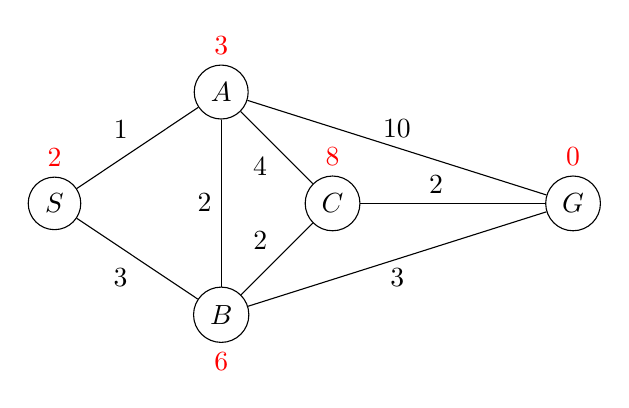
\begin{tikzpicture}
[node distance=2cm, main node/.style={circle,draw,minimum size=6mm},
every label/.style={red}]
\node[main node, label=above:{2}] (s) {$S$};
\node[main node, above right of=s, xshift=2em, label=above:{3}](a) {$A$};
\node[main node, below right of=s, xshift=2em, label=below:{6}] (b) {$B$};
\node[main node, below right of=a, label=above:{8}] (c) {$C$};
\node[main node, right of=c, xshift=3em, label=above:{0}] (g) {$G$};

\draw (s) -- node[above left] {1} (a);
\draw (s) -- node[below left] {3} (b);
\draw (a) -- node[left] {2} (b);
\draw (a) -- node[below left] {4} (c);
\draw (a) -- node[above] {10} (g);

\draw (b) -- node[above left] {2} (c);
\draw (b) -- node[below] {3} (g);
\draw (c) -- node[above left] {2} (g);
\end{tikzpicture}
\end{minipage}
\end{center}

\vspace{2em}
\begin{tabularx}{\textwidth}{|c|C|c|c|c|X|X|}\hline
   Iteration & Path & $g(n)$ & $h(n)$
   & $\begin{array}{c}
      f(n) =\\[-0.5em]g(n) + h(n)
   \end{array}$ 
   & Closed Fringe & Open Fringe \\\hline
   
   Initialize & $\begin{array}{l}S\end{array}$ & 0 & 2 & 2
   & $\{ \ \}$ &  $\{S(2)\}$ \\\hline
   
   1
   & \makecell{$S \to A$\\$S \to B$}
   & \makecell{0+1 = 1\\0+3 = 3} & \makecell{3\\6}
   & \makecell{4\\9}
   & $\{S\}$ &  $\{\ul[rgbRF]{A(4)},B(9)\}$\\\hline
   
   2
   & \makecell{$S \to A \to B$\\$S \to A \to C$\\$S \to A \to G$}
   & \makecell{1+2 = 3\\1+4 = 5\\1+10 = 11} & \makecell{6\\8\\0}
   & \makecell{9\\13\\\rgbR{11}}
   & $\{S,A\}$ &  $\{\ul[rgbRF]{B(9)},C(13),G(\rgbR{11})\}$\\\hline
   
   3
   & \makecell{$S \to A \to B \to C$\\$S \to A \to B \to G$}
   & \makecell{3+2 = 5\\3+3 = 6} & \makecell{8\\0}
   & \makecell{13\\\rgbR{6}}
   & $\{S,A,B\}$ &  $\{C(13),\ul[rgbRF]{G(\rgbR{6})}\}$\\\hline
\end{tabularx}

Since agent current \& goal state is same, hence the return path is: $S \to A \to B \to G$ \quad and \quad Path cost $=$ 6

\subsection{Admissible \& Consistent Heuristic}



\textbf{Admissible:}
A heuristic will be admissible at, \ $0 \leq h(n) \leq h*(n)$\\
\begin{tabular}{lll}
   where,& $h(n)$ &: heuristic value of node $n$ \\
         & $h*(n)$ &: optimal cost from node $n$ to goal node.
\end{tabular}

\textbf{Consistent:}
A heuristic will be consistent if, \ $\forall(A,B): 0 \leq h(S) - h(G) \leq \text{cost}(A,B)$\\
\begin{tabular}{lll}
   where,& $h(A)$ &: heuristic value of node $A$ \\
         & $h(B)$ &: heuristic value of node $B$ \\
         & cost$(A,B)$ &: path cost from node $A$ to node $B$.
\end{tabular}

\section{8 Puzzle Game}

\begin{minipage}[t]{0.5\textwidth}
\vspace{0pt}
Now, the number of steps required to reach the goal will definitely be greater than or equal to 4. Because every misplaced tile must be moved at least once.

\vspace{1em}
Thus, the heuristic function used never overestimates the cost to reach the goal. Hence, it is an admissible heuristic.
\end{minipage}%
\hfill
\begin{minipage}[t]{0.36\textwidth}
\vspace{0pt}
\begin{minipage}{3cm}
   \begin{tabular}{|c|c|c|}\hline
      \rgbR{2} & \rgbR{8} & 3 \\\hline
      \rgbR{1} & \rgbR{6} & 4 \\\hline
      7 & & 5 \\\hline
      \multicolumn{3}{c}{Initial State}
   \end{tabular}
\end{minipage}%
\begin{minipage}{3cm}
   \begin{tabular}{|c|c|c|}\hline
      1 & 2 & 3 \\\hline
      8 & & 4 \\\hline
      7 & 6 & 5 \\\hline
      \multicolumn{3}{c}{Final State}
   \end{tabular}
\end{minipage}

\vspace{1em}
$h_1$: Misplace tiles heuristic = 4

\vspace{0.5em}
$h_2$: Manhattan Distance Heuristic,\\[0.5em]
\begin{tabular}{|l|l|l|l|l|l|l|l|l}\cline{1-8}
   \rgbR{1} & \rgbR{2} & 3 & 4 & 5 & \rgbR{6} & 7 & \rgbR{8}\\\cline{1-8}
   1 & 1 & 0 & 0 & 0 & 1 & 0 & 2 & $h_1(S) $= 5\\\cline{1-8}
\end{tabular}
\end{minipage}%
